% =====================================================================
%  CS 6330 HW2 background: power law and exponential (Q&A note)
%  Build: latexmk -C && latexmk -xelatex p1_distributions.tex
% =====================================================================
\documentclass[11pt]{article}

\usepackage[letterpaper,margin=0.9in]{geometry}
\usepackage{fontspec}
\usepackage{xeCJK}
\setCJKmainfont{Apple SD Gothic Neo}
\xeCJKsetup{CJKspace=true}
\usepackage{amsmath}
\usepackage{xcolor}
\usepackage{graphicx}
\usepackage{booktabs}
\usepackage{tikz}
\usepackage{float}
\usepackage[colorlinks,linkcolor=blue!60!black,filecolor=blue!60!black,urlcolor=blue!60!black]{hyperref}
\usepackage{cleveref}

\newsavebox{\calloutbox}
\newenvironment{callout}[1][]
  {\par\medskip\noindent
   \begin{lrbox}{\calloutbox}\begin{minipage}{0.92\linewidth}
   \def\calloutttl{#1}\ifx\calloutttl\empty\else\textbf{#1}\par\smallskip\fi}
  {\end{minipage}\end{lrbox}%
   \fcolorbox{black!30}{black!3}{\usebox{\calloutbox}}\par\medskip}

\newcommand{\term}[1]{\textbf{#1}}
% Pointer from a note section to the matching lecture-note chapter
% (book_intro_2_ds/main.pdf). Numbers are from the 2026/09/28 build.
% Links into the lecture-note book PDF by hyperref destination name.
\newcommand{\bookpdf}{../../book_intro_2_ds/main.pdf}
\newcommand{\booksec}[1]{\href{\bookpdf\#section.#1}{\S#1}}
\newcommand{\bookch}[1]{\href{\bookpdf\#chapter.#1}{#1장}}
\newcommand{\lecnote}[1]{\par\noindent{\small\color{black!60}\textbf{강의 노트:} #1}\par\smallskip}
\setlength{\parindent}{0pt}
\setlength{\parskip}{0.5em}

\title{HW2 문제 1 배경: 멱법칙(Power Law)과 지수분포(Exponential)}
\author{Taek Lim}
\date{2026/09/28}

\begin{document}
\maketitle

% Overview first: people share vs amount share, then Lorenz, then the normal.
% (a),(b): alpha = 2.16, x_min = 1 (the 80/20 case, sec:pareto), E[X] = 7.25.
%   Axis u = log10 x. Heights are rescaled so each panel's total area is 1:
%   (a) people  ln10 * x f(x)       = 2.671  * 10^(-1.16 u)
%   (b) amount  ln10 * x^2 f(x)/E[X] = 0.3684 * 10^(-0.16 u)
%   The split x = 4 is u = 0.602.
% (c) airport points: cumulative route share of the sorted 01_airport_routes.csv
%     at every 5% of airports (computed with python, 2026/09/28).
\begin{figure}[H]
  \centering
  \begin{minipage}[b]{0.48\linewidth}
    \centering
    \begin{tikzpicture}[x=1.05cm,y=1.05cm]
      \fill[blue!15] (0,0) -- plot[domain=0:0.602,samples=30] (\x,{2.671*10^(-1.16*\x)}) -- (0.602,0) -- cycle;
      \fill[red!25] (0.602,0) -- plot[domain=0.602:6,samples=80] (\x,{2.671*10^(-1.16*\x)}) -- (6,0) -- cycle;
      \draw[thick,blue] plot[domain=0:6,samples=120] (\x,{2.671*10^(-1.16*\x)});
      \draw[->] (0,0) -- (6.4,0) node[right] {$x$};
      \draw[->] (0,0) -- (0,3.0) node[above] {사람};
      \foreach \u/\l in {0/1,1/10,2/10^2,4/10^4,6/10^6} \draw (\u,0.06) -- (\u,-0.06) node[below] {$\l$};
      \draw[dashed] (0.602,0) -- (0.602,2.6) node[above] {$4$};
      \node[blue!70!black,font=\small] at (1.9,1.6) {사람 80\%};
      \draw[->,blue!70!black] (1.4,1.45) -- (0.35,0.9);
      \node[red!70!black,font=\small] at (2.6,0.75) {사람 20\%};
      \draw[->,red!70!black] (2.1,0.6) -- (1.0,0.12);
    \end{tikzpicture}\\[2pt]
    {\small (a) 사람의 분포: $f(x)$}
  \end{minipage}\hfill
  \begin{minipage}[b]{0.48\linewidth}
    \centering
    \begin{tikzpicture}[x=1.05cm,y=7.3cm]
      \fill[blue!15] (0,0) -- plot[domain=0:0.602,samples=30] (\x,{0.3684*10^(-0.16*\x)}) -- (0.602,0) -- cycle;
      \fill[red!25] (0.602,0) -- plot[domain=0.602:6,samples=80] (\x,{0.3684*10^(-0.16*\x)}) -- (6,0) -- cycle;
      \draw[thick,blue] plot[domain=0:6,samples=120] (\x,{0.3684*10^(-0.16*\x)});
      \draw[->] (0,0) -- (6.4,0) node[right] {$x$};
      \draw[->] (0,0) -- (0,0.41) node[above] {양};
      \foreach \u/\l in {0/1,1/10,2/10^2,4/10^4,6/10^6} \draw (\u,0.008) -- (\u,-0.008) node[below] {$\l$};
      \draw[dashed] (0.602,0) -- (0.602,0.356) node[above] {$4$};
      \node[blue!70!black,font=\small] at (2.2,0.33) {양 20\%};
      \draw[->,blue!70!black] (1.75,0.32) -- (0.3,0.22);
      \node[red!70!black,font=\small] at (3.3,0.12) {양 80\% ($10^6$ 너머에 11\% 더)};
    \end{tikzpicture}\\[2pt]
    {\small (b) 양의 분포: $x \cdot f(x)$}
  \end{minipage}

  \bigskip
  \begin{minipage}[b]{0.48\linewidth}
    \centering
    \begin{tikzpicture}[x=4.6cm,y=4.6cm]
      \draw[->] (0,0) -- (1.08,0);
      \node[font=\small] at (0.5,-0.16) {사람 누적 비율 (적게 가진 쪽부터)};
      \draw[->] (0,0) -- (0,1.08) node[above] {양 누적 비율};
      \foreach \t in {0.2,0.8,1} \draw (\t,0.015) -- (\t,-0.015) node[below] {\t};
      \foreach \v in {0.2,0.8,1} \draw (0.015,\v) -- (-0.015,\v) node[left] {\v};
      \draw[black!40,dotted,thick] (0,0) -- (1,1);
      \draw[orange!80!black,thick,dash dot] plot coordinates {(0.00,0.000) (0.05,0.003) (0.10,0.005)
        (0.15,0.008) (0.20,0.010) (0.25,0.015) (0.30,0.020) (0.35,0.025) (0.40,0.031) (0.45,0.038)
        (0.50,0.047) (0.55,0.057) (0.60,0.069) (0.65,0.084) (0.70,0.102) (0.75,0.127) (0.80,0.162)
        (0.85,0.214) (0.90,0.301) (0.95,0.470) (1.00,1.000)};
      % Pareto Lorenz curve L(p) = 1 - (1-p)^{(alpha-2)/(alpha-1)}, alpha = 2.16
      \draw[thick,blue] plot[domain=0:0.9999,samples=120] (\x,{1-(1-\x)^(0.138)});
      \draw[dashed] (0.8,0) -- (0.8,0.2) -- (0,0.2);
      \draw[red,line width=2pt] (1,0.2) -- (1,1);
      \fill (0.8,0.2) circle (1.2pt);
      \node[right,font=\small,red!70!black] (t1) at (0.05,0.95) {상위 20\% $\to$ 양 80\%};
      \node[right,font=\small] (t2) at (0.05,0.8) {하위 80\% $\to$ 양 20\%};
      \draw[->,red!70!black] (t1.east) -- (0.97,0.6);
      \draw[->] (t2.south) -- (0.78,0.22);
    \end{tikzpicture}\\[2pt]
    {\small (c) 로렌츠 곡선(Lorenz Curve)}
  \end{minipage}\hfill
  \begin{minipage}[b]{0.48\linewidth}
    \centering
    \begin{tikzpicture}[x=0.75cm,y=6cm]
      \draw[->] (-3.3,0) -- (3.5,0) node[right] {$x$};
      \draw[->] (0,0) -- (0,0.5) node[above] {$f(x)$};
      \foreach \t in {-2,0,2} \draw (\t,0.01) -- (\t,-0.01) node[below] {\t};
      \draw[thick,black!60,dashed] plot[domain=-3:3,samples=80] (\x,{0.3989*exp(-\x*\x/2)});
      \node[right,black!60] at (0.9,0.34) {$\mu$에서 대칭};
    \end{tikzpicture}\\[2pt]
    {\small (d) 정규분포(Normal), $\mu = 0$, $\sigma = 1$}
  \end{minipage}
  \caption{멱법칙의 80/20을 사람과 양으로 나눠 본 그림, 그리고 정규분포. 읽는 법은 아래 목록.}
  \label{fig:overview}
\end{figure}

\paragraph{\Cref{fig:overview} 읽는 법.}
\begin{description}
  \item[(a), (b) 같은 멱법칙] $f(x) = 1.16\,x^{-2.16}$, $x_{\min} = 1$.
    \begin{itemize}
      \item 가로축은 로그 눈금이다 ($1, 10, 10^2, \dots$). 꼬리가 길어 보통 눈금에는 다 들어가지 않는다.
      \item 두 패널 모두 전체 넓이 = 1 (100\%). 넓이가 곧 비율이다.
      \item 파란 면: $x < 4$. 빨간 면: $x \ge 4$.
    \end{itemize}
  \item[(a) 사람의 분포] 넓이 = $\int f(x)\,dx$ = \term{사람의 비율}.
    \begin{itemize}
      \item 파란 면: 사람의 80\%.
      \item 빨간 면: 사람의 20\%.
    \end{itemize}
  \item[(b) 양의 분포] 넓이 = $\int x\,f(x)\,dx$ = \term{양의 비율}.
    \begin{itemize}
      \item 같은 사람들인데 넓이가 뒤집힌다. 파란 면: 양의 20\%.
      \item 빨간 면: 양의 80\%. 값 $x$를 곱해 큰 $x$ 쪽이 무거워졌다.
    \end{itemize}
  \item[(c) 로렌츠 곡선] (a)와 (b)를 한 곡선으로 합친 것. 넓이가 아니라 \term{높이}로 읽는다.
    \begin{itemize}
      \item 가로축: 사람의 누적 비율 (적게 가진 사람부터).
      \item 세로축: 그 사람들이 가진 양의 누적 비율.
      \item 파란 실선: (a), (b)의 멱법칙.
      \item 주황 일점쇄선: 실제 공항 노선 데이터.
      \item 회색 점선: 모두가 같은 양을 가질 때 ($y = x$).
      \item 검은 점 $(0.8, 0.2)$: 하위 80\%가 양의 20\%를 가진다.
      \item 빨간 굵은 선: 상위 20\%가 양의 80\%를 가진다 (\Cref{sec:pareto}).
      \item 공항 데이터: 하위 80\%가 양의 16.2\%를 가진다.
    \end{itemize}
  \item[(d) 표준정규분포 PDF] 회색 점선, $\mu = 0$, $\sigma = 1$.
    \begin{itemize}
      \item 평균을 가운데 두고 좌우 대칭이다.
      \item 평균에서 멀어지면 매우 빨리 $0$이 된다.
    \end{itemize}
\end{description}

\begin{callout}[질문]
Suppose the given data points follow a power law distribution: what is power
law distribution? and alpha?
\end{callout}

% =====================================================================
\section{멱법칙 분포란}
\label{sec:what}
\lecnote{\bookch{4} ``분포'' \booksec{4.4} 멱법칙 (\texttt{04-distributions.tex}, deck 6 slide 19--22). 요약 표는 \booksec{4.8}.}

\term{멱법칙}(Power Law) 분포는 소수의 큰 값이 전체의 대부분을 차지하는
분포다. 대부분의 관측값은 작다. 아주 큰 값은 드물지만, 정규분포(Normal)나
지수분포(Exponential)보다 \term{훨씬 자주} 나온다. 이 성질을
\term{꼬리가 두껍다}(Heavy Tail)고 한다.

\term{파레토 분포}(Pareto Distribution), ``80/20 법칙''이라고도 부른다.
예: 공항별 노선 수, 도시 인구, 단어 빈도, 부의 분포.

확률밀도함수(PDF)는 다음과 같다.
\begin{equation}
  f(x) = \frac{\alpha - 1}{x_{\min}}
         \left(\frac{x}{x_{\min}}\right)^{-\alpha},
  \qquad x \ge x_{\min},\ \alpha > 1
  \label{eq:pdf}
\end{equation}

\begin{itemize}
  \item $x_{\min}$: 멱법칙이 성립하기 시작하는 하한.
  \item $\alpha$: 지수(Power Law Exponent). 꼬리가 얼마나 빨리 줄어드는지 정한다.
  \item 앞의 $\frac{\alpha-1}{x_{\min}}$는 전체 넓이를 $1$로 맞추는 정규화 상수다.
\end{itemize}

\Cref{fig:powerlaw-pdf}는 $x_{\min} = 1$에서 $\alpha$만 바꾼 세 곡선이다.
모두 $x_{\min}$에서 가장 높고 오른쪽으로 줄어든다.

\begin{figure}[H]
  \centering
  \begin{tikzpicture}[x=2.2cm,y=1.6cm]
    \draw[->] (0,0) -- (5.3,0) node[right] {$x$};
    \draw[->] (0,0) -- (0,2.8) node[above] {$f(x)$};
    \foreach \t in {1,...,5} \draw (\t,0.05) -- (\t,-0.05) node[below] {\t};
    \foreach \v in {1,2} \draw (0.05,\v) -- (-0.05,\v) node[left] {\v};
    \draw[dotted] (1,0) -- (1,2.5);
    \node[below left] at (1,-0.25) {$x_{\min}$};
    % f(x) = (alpha - 1) x^{-alpha}, x_min = 1
    \draw[thick,blue] plot[domain=1:5,samples=80] (\x,{0.5*\x^(-1.5)});
    \draw[thick,red,dashed] plot[domain=1:5,samples=80] (\x,{1.5*\x^(-2.5)});
    \draw[thick,green!50!black,dash dot] plot[domain=1:5,samples=80] (\x,{2.5*\x^(-3.5)});
    % legend
    \begin{scope}[shift={(3.2,2.4)}]
      \draw[thick,blue] (0,0) -- (0.3,0) node[right,black] {$\alpha = 1.5$};
      \draw[thick,red,dashed] (0,-0.3) -- (0.3,-0.3) node[right,black] {$\alpha = 2.5$};
      \draw[thick,green!50!black,dash dot] (0,-0.6) -- (0.3,-0.6)
        node[right,black] {$\alpha = 3.5$};
    \end{scope}
  \end{tikzpicture}
  \caption{멱법칙 PDF $f(x) = (\alpha - 1)\,x^{-\alpha}$ ($x_{\min} = 1$).
  파란 실선 $\alpha = 1.5$, 빨간 점선 $\alpha = 2.5$, 초록 일점쇄선 $\alpha = 3.5$.
  $\alpha$가 클수록 $x_{\min}$ 근처에 몰리고 꼬리가 빨리 줄어든다.
  $\alpha$가 작을수록 꼬리가 두꺼워 $x = 5$에서도 높이가 남는다.}
  \label{fig:powerlaw-pdf}
\end{figure}

\subsection{정규화 상수: 곡선 아래 넓이 $= 1$}
\label{sec:normalize}

\begin{callout}[질문]
앞의 $\frac{\alpha-1}{x_{\min}}$는 전체 넓이를 $1$로 맞추는 정규화 상수다.
>> area below distribution line => 1?
\end{callout}

그렇다. PDF 곡선 아래 전체 넓이는 ``어떤 값이든 하나는 나올 확률''이므로
반드시 $1$이다.
\[
  \int_{x_{\min}}^{\infty} f(x)\,dx = 1
  \qquad \text{(모든 PDF의 조건)}
\]
$x^{-\alpha}$만으로는 넓이가 $1$이 아니다. 그래서 앞에 상수 $C$를 곱해
넓이를 $1$로 맞춘다. 이 $C$가 \term{정규화 상수}(Normalization Constant)다.

\paragraph{$C$ 구하기.} $x^{-\alpha}$의 넓이를 먼저 구한다.
\begin{align*}
  \int_{x_{\min}}^{\infty} x^{-\alpha}\,dx
    &= \left[\frac{x^{1-\alpha}}{1-\alpha}\right]_{x_{\min}}^{\infty}
    && \text{거듭제곱 적분}\\
    &= 0 - \frac{x_{\min}^{1-\alpha}}{1-\alpha}
    && \text{$\alpha > 1$이면 $x \to \infty$에서 $x^{1-\alpha} \to 0$}\\
    &= \frac{x_{\min}^{1-\alpha}}{\alpha-1}
    && \text{부호 정리}
\end{align*}
넓이가 $1$이 되려면 $C$는 이 값의 역수다.
\begin{align*}
  C &= (\alpha-1)\,x_{\min}^{\alpha-1}
    && \text{넓이의 역수}\\
  f(x) = C\,x^{-\alpha}
    &= \frac{\alpha-1}{x_{\min}} \left(\frac{x}{x_{\min}}\right)^{-\alpha}
    && \text{$x_{\min}^{\alpha-1} x^{-\alpha} = \tfrac{1}{x_{\min}}(x/x_{\min})^{-\alpha}$}
\end{align*}
\Cref{eq:pdf}와 같다. 둘째 줄에서 $\alpha > 1$이 쓰였다. $\alpha \le 1$이면 넓이가
무한대라 어떤 $C$로도 $1$을 만들 수 없다. 이것이 $\alpha > 1$ 조건의 이유다.

\paragraph{예제.} $\alpha = 2.5$, $x_{\min} = 1$.
\begin{align*}
  &\int_1^{\infty} x^{-2.5}\,dx = \frac{1}{1.5} = 0.667 && \text{상수 없이 넓이}\\
  &C = 1.5                                             && \text{역수}\\
  &1.5 \times 0.667 = 1                                && \text{곱하면 넓이 $1$}
\end{align*}

\begin{figure}[H]
  \centering
  \begin{tikzpicture}[x=2.2cm,y=1.6cm]
    \fill[red!15] (1,0) -- plot[domain=1:5,samples=80] (\x,{1.5*\x^(-2.5)}) -- (5,0) -- cycle;
    \draw[->] (0,0) -- (5.3,0) node[right] {$x$};
    \draw[->] (0,0) -- (0,1.8) node[above] {$f(x)$};
    \foreach \t in {1,...,5} \draw (\t,0.05) -- (\t,-0.05) node[below] {\t};
    \foreach \v in {0.5,1,1.5} \draw (0.05,\v) -- (-0.05,\v) node[left] {\v};
    \draw[thick,red,dashed] plot[domain=1:5,samples=80] (\x,{1.5*\x^(-2.5)});
    \node[right] at (1.6,0.8) {색칠한 넓이 $= 1$ ($x \to \infty$까지)};
  \end{tikzpicture}
  \caption{$\alpha = 2.5$, $x_{\min} = 1$의 멱법칙 PDF $f(x) = 1.5\,x^{-2.5}$
  (빨간 점선). 빨간 면이 곡선 아래 넓이다. $x = 5$ 너머 꼬리까지 합치면
  정확히 $1$이다.}
  \label{fig:powerlaw-area}
\end{figure}

\subsection{PDF는 어디서 왔나}
\label{sec:pdf-origin}

\begin{callout}[질문]
how did you get pdf for pwer law? is it normal? and why we call pareto
distribution? buecaseu 80 normal 20 outlaw? whats its graph look like? can i
have a figure at the begiging?
\end{callout}

만든 식이 아니라 \term{멱법칙의 정의}에서 나온다. 멱법칙은 ``확률이 $x$의
거듭제곱으로 줄어든다''는 가정 하나다.
\[
  f(x) \propto x^{-\alpha}
  \qquad \text{($\propto$: 상수배를 빼면 같다)}
\]
이 가정에 빠진 것은 상수 하나뿐이고, 넓이를 $1$로 맞추면 정해진다
(\Cref{sec:normalize}). 그 결과가 \Cref{eq:pdf}다. 강의 노트(deck 6
slide 19--22)와 Clauset et al.\ (2009)이 쓰는 표준형(연속형)이 이것이다.

\paragraph{다른 길: 여집합 CDF에서 미분.} 파레토는 ``$x$보다 큰 값의 비율''로
정의했다. 여기서 시작해도 같은 식이 나온다.
\begin{align*}
  P(X \ge x) &= \left(\frac{x}{x_{\min}}\right)^{-(\alpha-1)}
    && \text{$x$보다 큰 비율 (\Cref{sec:alpha}의 기울기 $-(\alpha-1)$)}\\
  f(x) &= -\frac{d}{dx} P(X \ge x)
    && \text{PDF는 CDF의 기울기}\\
       &= (\alpha-1) \left(\frac{x}{x_{\min}}\right)^{-\alpha} \cdot \frac{1}{x_{\min}}
    && \text{거듭제곱 미분, 지수가 $1$ 줄었다}
\end{align*}
\Cref{eq:pdf}와 같다.

\subsection{정규분포인가}
\label{sec:not-normal}
아니다. 정규분포(Normal)와 모양이 정반대에 가깝다(\Cref{fig:overview}).

\begin{table}[H]
  \centering
  \caption{멱법칙과 정규분포 비교}
  \label{tab:pl-vs-normal}
  \begin{tabular}{lll}
    \toprule
    & 멱법칙(Power Law) & 정규분포(Normal) \\
    \midrule
    가장 높은 곳 & $x_{\min}$ (맨 왼쪽) & 평균 $\mu$ (가운데) \\
    \midrule
    모양 & 한쪽으로만 줄어듦 & 좌우 대칭 종 모양 \\
    \midrule
    값의 범위 & $x \ge x_{\min} > 0$ & 모든 실수 \\
    \midrule
    꼬리 & $x^{-\alpha}$, 느리게 줄어듦 & $e^{-x^2/2}$, 매우 빨리 줄어듦 \\
    \midrule
    평균이 대표값인가 & 아니다 (소수가 끌어올림) & 그렇다 (평균 = 중앙값) \\
    \bottomrule
  \end{tabular}
\end{table}

\paragraph{예제: 공항 노선 수.} 평균과 중앙값이 크게 다르다.
\begin{align*}
  &\bar x = 19.8                && \text{평균}\\
  &\text{중앙값} = 4            && \text{절반의 공항은 노선 4개 이하}\\
  &82\%                         && \text{평균보다 작은 공항의 비율}
\end{align*}
정규분포라면 평균 아래가 절반(50\%)이어야 한다.

\subsection{왜 파레토 분포라고 부르나}
\label{sec:pareto}
이탈리아 경제학자 빌프레도 파레토(Vilfredo Pareto)의 이름이다. 그는 1890년대에
소득이 $x$ 이상인 사람의 수가 $x$의 거듭제곱으로 줄어든다는 것을 관찰했다.
흔히 전하는 예가 ``이탈리아 땅의 80\%를 인구 20\%가 가진다''이다. ``80/20 법칙''
(Pareto Principle)이라는 이름은 뒤에 품질 관리 분야의 조셉 주란(Joseph Juran)이 붙였다.

\paragraph{``80 정상, 20 이상치''가 아니다.} 80/20은 \term{사람의 20\%가 전체 양의
80\%를 가진다}는 뜻이다. 20\%는 버릴 이상치가 아니라 분포의 핵심인 긴 꼬리다
(\Cref{fig:overview}(a), (b)의 빨간 면).

\begin{callout}[질문]
가진 양이 그래프 아래면적을 이야기 하는거야? 그런데 그림 상으로 80퍼센트 사람이
가진 양이 20퍼센트로 안 보여 스케일 다르게 해서 보여줘야 하는 거아니야?
\end{callout}

\paragraph{PDF 아래 넓이는 사람의 비율이지 양이 아니다.} 두 넓이를 구별해야 한다.
\begin{align*}
  &\int_a^b f(x)\,dx       && \text{$a$와 $b$ 사이에 있는 \term{사람의 비율}}\\
  &\int_a^b x\,f(x)\,dx    && \text{그 사람들이 가진 \term{양} (값 $x$를 곱했다)}
\end{align*}
\Cref{fig:overview}(a)의 넓이는 첫째 줄, (b)의 넓이는 둘째 줄이다. 그래서 파란 면이 커 보이는 것이 맞다.
사람은 80\%가 거기 있다. 양은 둘째 줄인데, 큰 $x$가 곱해지므로 꼬리 쪽 무게가 커진다.
그 양의 대부분은 그림 오른쪽 끝($x = 10$) 너머 먼 꼬리에 있다.
\begin{align*}
  &\int_4^{10} x f(x)\,dx \big/ E[X] = 0.11 && \text{그림에 보이는 빨간 구간의 양}\\
  &0.80 - 0.11 = 0.69                       && \text{$x > 10$에 있는 양}
\end{align*}
보통 눈금으로는 꼬리가 잘린다. 그래서 \Cref{fig:overview}는 가로축을 로그 눈금으로
바꾸고, (a) 사람과 (b) 양을 같은 축에 나란히 그렸다. 두 비율을 한 곡선으로 합치면
(c)의 \term{로렌츠 곡선}(Lorenz Curve)이 된다. 넓이가 아니라
\term{높이}로 읽는다. 가로 $0.8$에서 곡선 높이가 $0.2$면 하위 80\%가 20\%를 가진 것이다.

\paragraph{80/20은 $\alpha$ 하나에서만 정확하다.} 상위 비율 $p$가 가진 양의 몫은
$\alpha > 2$일 때 다음과 같다.
\[
  \text{몫} = p^{(\alpha-2)/(\alpha-1)}
  \qquad \text{($x \cdot f(x)$를 꼬리에서 적분해 평균으로 나눈 값)}
\]
\begin{align*}
  &\alpha = 2.16,\ p = 0.2              && \text{가정}\\
  &(2.16-2)/(2.16-1) = 0.138            && \text{지수}\\
  &0.2^{0.138} = 0.80                   && \text{상위 20\%가 80\%를 가진다}
\end{align*}
$\alpha$가 $2$에 가까워지면 몫은 $1$(100\%)로 가고, $\alpha$가 커지면 줄어든다.
그래서 ``80/20''은 멱법칙의 한 예일 뿐 모든 멱법칙의 성질은 아니다.

\paragraph{예제: 공항 데이터.} 노선이 많은 순으로 상위 20\%를 센다.
\begin{align*}
  &3409 \times 0.2 = 682          && \text{상위 20\% 공항 수}\\
  &83.8\%                         && \text{그 682곳이 가진 노선의 몫}
\end{align*}
실제 데이터가 거의 80/20이다. 적합한 $\hat\alpha = 1.612 < 2$(\Cref{sec:p1a})로는
몫이 100\%에 가까워야 하는데, 실제 데이터는 큰 값에서 끊기기(Cutoff) 때문에
83.8\%에서 멈춘다.

% =====================================================================
\section{$\alpha$의 의미}
\label{sec:alpha}
\lecnote{\booksec{4.4} 멱법칙 (로그-로그 그림, deck 6 slide 22). 평균과 분산의 조건은 \booksec{4.8} 요약 표의 ``조건부 존재'' 칸.}

\subsection{꼬리의 두께}
$\alpha$가 \term{작을수록} 꼬리가 두꺼워 극단값이 더 자주 나온다.
$\alpha$가 \term{클수록} 꼬리가 빨리 줄어든다.

\subsection{$\alpha$에 걸린 조건}
\begin{itemize}
  \item $\alpha > 1$: 넓이가 $1$이 되려면(확률분포가 되려면) 필요하다.
  \item $\alpha > 2$: 이때만 평균이 유한하다.
        $E[X] = \frac{\alpha-1}{\alpha-2}\,x_{\min}$.
  \item $\alpha > 3$: 이때만 분산이 유한하다.
\end{itemize}
실제 데이터는 흔히 $2 < \alpha < 3$이다. 평균은 있어도 분산이 발산하는
경우가 많다.

\begin{callout}[질문]
2.2 $\alpha$에 걸린 조건 (위 세 줄): explain more on this
\end{callout}

\subsubsection{핵심 도구: $x^{-p}$의 넓이는 언제 유한한가}
세 조건은 모두 한 가지 사실에서 나온다.
\[
  \int_{1}^{\infty} x^{-p}\,dx
  = \begin{cases}
      \dfrac{1}{p-1} & p > 1 \quad \text{(유한)}\\[4pt]
      \infty         & p \le 1 \quad \text{(발산)}
    \end{cases}
\]
곡선이 $x^{-p}$로 줄어들 때, $p$가 $1$보다 커야 꼬리가 충분히 빨리 줄어
넓이가 유한하다. $p = 1$이 경계다.
\begin{align*}
  &\int_1^{1000} x^{-1}\,dx = \ln 1000 = 6.9       && \text{$p = 1$: 구간을 늘리면}\\
  &\int_1^{10^6} x^{-1}\,dx = \ln 10^6 = 13.8      && \text{넓이가 끝없이 커진다}\\
  &\int_1^{\infty} x^{-2}\,dx = 1                  && \text{$p = 2$: 유한}
\end{align*}

\subsubsection{평균과 분산은 넓이 계산이다}
평균과 분산도 적분이다. 적분 안에 $x$를 한 번, 두 번 더 곱할 뿐이다.
\begin{align*}
  E[X]   &= \int_{x_{\min}}^{\infty} x \cdot C x^{-\alpha}\,dx
          = C \int_{x_{\min}}^{\infty} x^{-(\alpha-1)}\,dx
         && \text{$x$를 한 번 곱했다: $p = \alpha - 1$}\\
  E[X^2] &= \int_{x_{\min}}^{\infty} x^2 \cdot C x^{-\alpha}\,dx
          = C \int_{x_{\min}}^{\infty} x^{-(\alpha-2)}\,dx
         && \text{두 번 곱했다: $p = \alpha - 2$}
\end{align*}
$x$를 곱할 때마다 지수 $p$가 $1$씩 줄어 꼬리가 느려진다. 각각에 ``$p > 1$''을 쓴다.

\begin{table}[H]
  \centering
  \caption{$x^k$를 곱한 적분이 유한해지는 조건. $k$는 곱한 횟수.}
  \label{tab:moments}
  \begin{tabular}{llll}
    \toprule
    구하는 것 & 적분 안의 꼬리 & 유한 조건 $p > 1$ & 결론 \\
    \midrule
    전체 넓이 ($k = 0$) & $x^{-\alpha}$     & $\alpha > 1$     & 확률분포가 된다 \\
    \midrule
    평균 $E[X]$ ($k = 1$) & $x^{-(\alpha-1)}$ & $\alpha - 1 > 1$ & $\alpha > 2$ \\
    \midrule
    $E[X^2]$ ($k = 2$)    & $x^{-(\alpha-2)}$ & $\alpha - 2 > 1$ & $\alpha > 3$ \\
    \bottomrule
  \end{tabular}
\end{table}

분산은 $\mathrm{Var}[X] = E[X^2] - (E[X])^2$이므로 $E[X^2]$가 유한해야 유한하다.
그래서 분산의 조건은 $\alpha > 3$이다.

\subsubsection{유한할 때의 값}
$C = (\alpha-1)\,x_{\min}^{\alpha-1}$(\Cref{sec:normalize})를 넣고 적분하면 다음과 같다.
\begin{align*}
  E[X]   &= \frac{\alpha-1}{\alpha-2}\,x_{\min}   && \alpha > 2\\
  E[X^2] &= \frac{\alpha-1}{\alpha-3}\,x_{\min}^2 && \alpha > 3\\
  \mathrm{Var}[X] &= \frac{\alpha-1}{(\alpha-2)^2(\alpha-3)}\,x_{\min}^2 && \alpha > 3
\end{align*}
분모의 $\alpha - 2$, $\alpha - 3$이 $0$에 가까워지면 값이 무한대로 커진다.
식 모양에도 조건이 드러난다.

\paragraph{예제 1: $\alpha = 4$, $x_{\min} = 1$ (셋 다 유한).}
\begin{align*}
  &E[X] = 3/2 = 1.5                && \text{평균}\\
  &E[X^2] = 3/1 = 3                && \text{제곱의 평균}\\
  &\mathrm{Var}[X] = 3 - 1.5^2 = 0.75 && \text{분산 (공식으로도 $3/(4 \cdot 1) = 0.75$)}
\end{align*}

\paragraph{예제 2: $\alpha = 2.5$, $x_{\min} = 1$ (평균만 유한).}
\begin{align*}
  &E[X] = 1.5/0.5 = 3   && \text{평균은 유한}\\
  &\alpha - 2 = 0.5 \le 1 && \text{$E[X^2]$의 꼬리 $x^{-0.5}$: 발산, 분산은 무한}
\end{align*}

\subsubsection{데이터 분석에서 뜻하는 것}
``평균이 무한''은 실제 데이터의 평균이 무한대라는 뜻이 아니다. 유한한 표본의
평균은 언제나 숫자 하나로 계산된다. 뜻하는 것은 \term{표본 평균이 한 값으로
수렴하지 않는다}는 것이다. 표본을 늘릴수록 전보다 더 큰 극단값이 들어와
표본 평균이 계속 뛴다.
\begin{itemize}
  \item $\alpha > 3$: 평균, 분산 모두 안정. 표본을 늘리면 정해진 값에 다가간다.
  \item $2 < \alpha \le 3$: 표본 평균은 수렴하지만, 표본 분산(표준편차)은 표본이
        커질수록 계속 커진다. 평균 $\pm$ 표준편차 같은 요약이 믿을 만하지 않다.
  \item $1 < \alpha \le 2$: 표본 평균조차 수렴하지 않는다. 평균보다 중앙값(Median)이
        나은 요약이다.
\end{itemize}
문제 1(a)의 공항 데이터는 $\hat\alpha = 1.612$로 마지막 경우다(\Cref{sec:p1a}).

\subsection{로그-로그 축에서 직선}
\Cref{eq:pdf}의 양변에 로그를 취한다.
\begin{align*}
  f(x) &= C\,x^{-\alpha}
       && \text{상수를 $C$로 묶었다}\\
  \log f(x) &= \log C - \alpha \log x
       && \text{양변에 로그}
\end{align*}
$\log x$에 대해 일차식이다. 그래서 \term{로그-로그 축에서 기울기가
$-\alpha$인 직선}이 된다. 지수분포는 같은 축에서 아래로 휘는 곡선이다
(\Cref{fig:loglog}). 이것으로 둘을 구별한다.

여집합 CDF $P(X \ge x)$로 그리면 기울기는 $-(\alpha - 1)$이다. 적분하면서
지수가 하나 줄기 때문이다.

\begin{figure}[H]
  \centering
  \begin{tikzpicture}[x=3.2cm,y=0.55cm]
    \draw[->] (0,0) -- (1.45,0) node[right] {$\log_{10} x$};
    \draw[->] (0,0) -- (0,-9.5) node[below] {$\log_{10} f(x)$};
    \foreach \u in {0,0.5,1} \draw (\u,0.1) -- (\u,-0.1) node[above=3pt] {\u};
    \foreach \v in {-2,-4,-6,-8} \draw (0.03,\v) -- (-0.03,\v) node[left] {\v};
    % power law, alpha = 2.5: straight line
    \draw[thick,blue] plot[domain=0:1.3,samples=2] (\x,{-2.5*\x});
    \node[blue,right] at (1.3,-3.25) {멱법칙, $\alpha=2.5$ (직선)};
    % exponential e^{-x}: log10 f = -x / ln 10 with x = 10^u
    \draw[thick,red,dashed] plot[domain=0:1.3,samples=60]
      (\x,{-0.4343*10^\x});
    \node[red,right] at (1.3,-8.7) {지수분포 $e^{-x}$ (아래로 휨)};
  \end{tikzpicture}
  \caption{로그-로그 축에서 멱법칙(파란 실선)과 지수분포(빨간 점선).
  멱법칙은 기울기 $-\alpha$의 직선, 지수분포는 아래로 휘는 곡선이다.}
  \label{fig:loglog}
\end{figure}

% =====================================================================
\section{데이터에서 $\alpha$ 추정하기}
\label{sec:estimate}
\lecnote{\bookch{10} ``과제 2'' \booksec{10.2} 모수 추정 (\texttt{hw02-data-distributions.tex}, 멱법칙 MLE 예제).}

최대우도추정(MLE, Maximum Likelihood Estimation; Clauset et al.\ 2009)을 쓴다.
\begin{equation}
  \hat\alpha = 1 + \frac{n}{\sum_{i=1}^{n} \ln(x_i / x_{\min})}
  \label{eq:mle}
\end{equation}
HW2 코드(\texttt{hw2/code/p1.py}의 \texttt{fit\_power\_law})도 이 식을 쓰고,
$x_{\min}$은 데이터의 최솟값으로 둔다.

로그-로그 히스토그램에 직선을 그어 기울기를 읽는 방법은 편향이 커서
권장하지 않는다. 직선이 맞는지 눈으로 확인하는 용도로만 쓴다.

\paragraph{예제.} 데이터 $\{1, 2, 4, 8\}$, $x_{\min} = 1$, $n = 4$.
\begin{align*}
  &\ln(1/1) = 0      && \\
  &\ln(2/1) = 0.693  && \\
  &\ln(4/1) = 1.386  && \\
  &\ln(8/1) = 2.079  && \\
  &0 + 0.693 + 1.386 + 2.079 = 4.159 && \text{분모 (로그의 합)}\\
  &1 + 4 / 4.159 = 1.962             && \text{$\hat\alpha$}
\end{align*}
$\hat\alpha \approx 1.96 < 2$이므로, 이 모형에서는 평균이 유한하지 않다.

% =====================================================================
\section{HW2 문제 1(a): 공항 노선 수 데이터}
\label{sec:p1a}
\lecnote{\booksec{10.4} 공항 노선 수, \booksec{10.3} 네 모형을 비교하는 방법. KS 거리는 \bookch{8} \booksec{8.8}, Q-Q 플롯은 \bookch{5} \booksec{5.5}.}

\begin{callout}[문제 1(a)]
What is the $\alpha$ if the distribution is power law?
\end{callout}

\Cref{eq:mle}를 공항별 노선 수 데이터(\texttt{01\_airport\_routes.csv})에
적용한다. 보고서의 답은 다음과 같다.
\begin{align*}
  &n = 3409               && \text{공항 수}\\
  &x_{\min} = 1           && \text{데이터의 최솟값 (노선 1개)}\\
  &\hat\alpha = 1.612     && \text{\Cref{eq:mle}의 결과}
\end{align*}

\subsection{$\hat\alpha = 1.612$가 뜻하는 것}
$1 < \hat\alpha < 2$이다. \Cref{sec:alpha}의 조건에 따라 확률분포는 되지만,
이 모형에서는 평균도 분산도 유한하지 않다. 그래서 모형에서 뽑은 표본은
노선이 $10^4$에서 $10^5$개인 공항까지 만들어 낸다. 실제 데이터는 최대
$915$에서 멈춘다.

\subsection{적합이 맞는 범위}
\begin{itemize}
  \item 노선 $1$개에서 약 $60$개까지: 여집합 CDF가 데이터와 겹치고,
        QQ 점이 $y = x$ 위에 놓인다.
  \item 약 $100$개 이상: 데이터는 아래로 휘며 끊기고(Cutoff), 모형은 직선으로
        계속 간다.
  \item KS 거리(Kolmogorov--Smirnov Distance) $D = 0.209$로 네 모형
        (멱법칙, 지수, 균등, 정규) 중 가장 작다.
\end{itemize}

\begin{figure}[H]
  \centering
  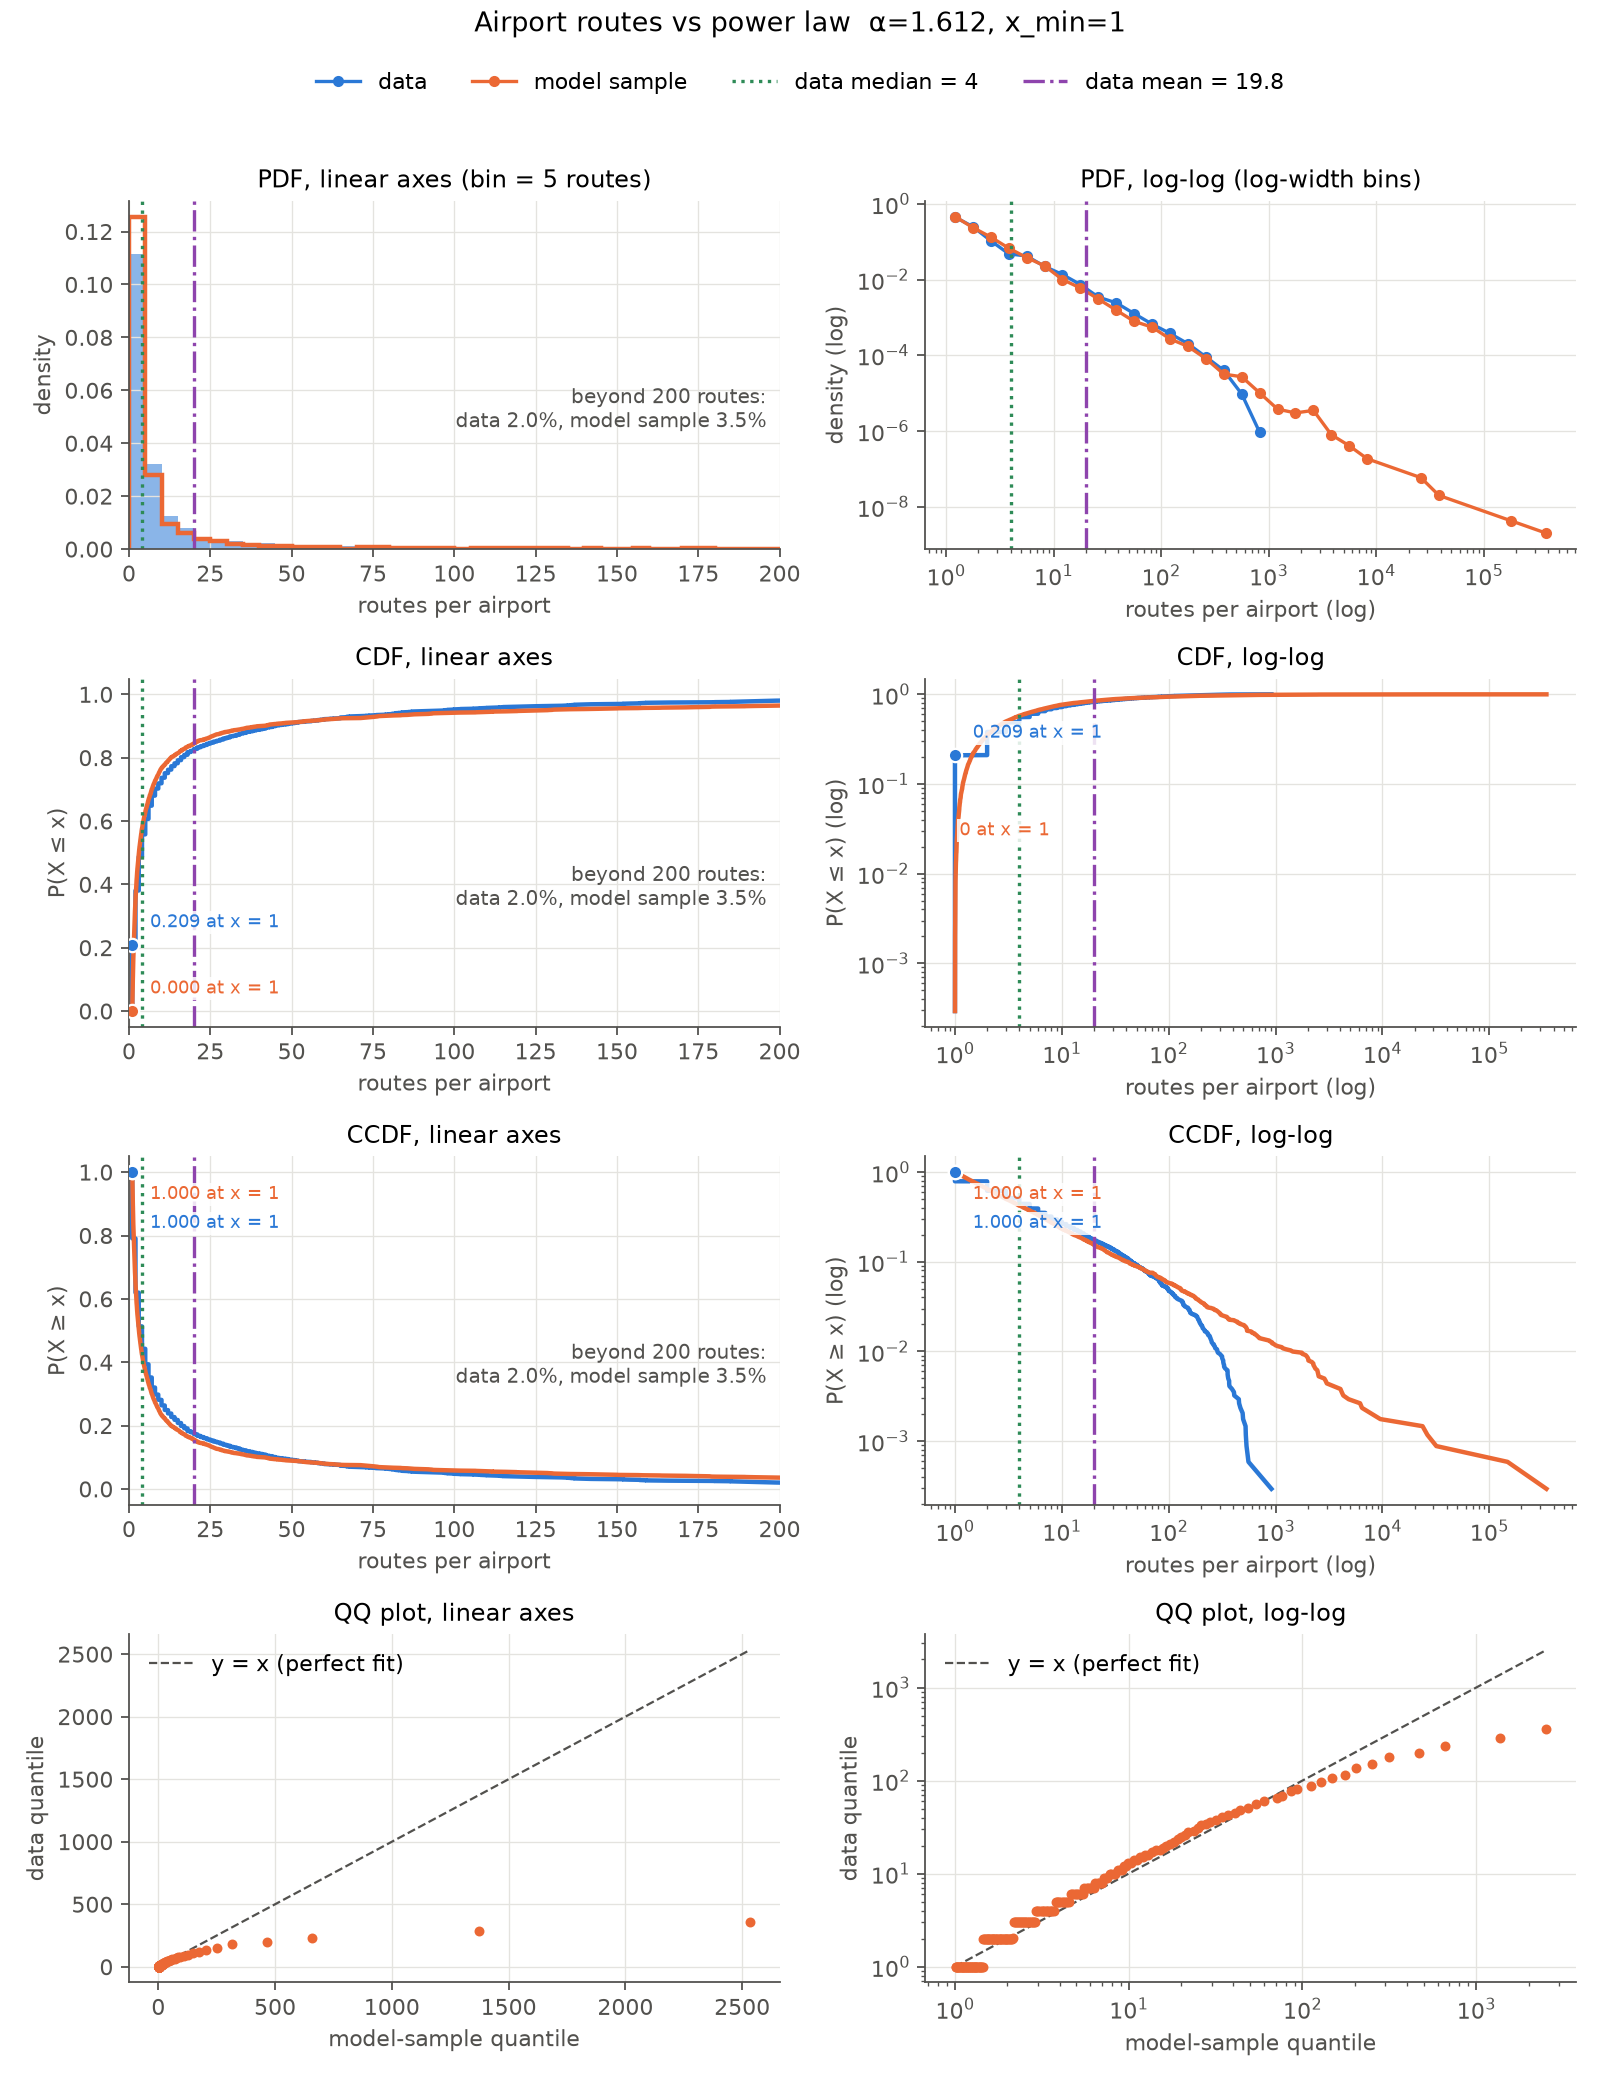
\includegraphics[width=\linewidth]{../figures/p1a_1_powerlaw.png}
  \caption{공항 노선 수에 멱법칙($\hat\alpha = 1.612$, $x_{\min} = 1$)을
  적합한 결과 (\texttt{code/p1.py}가 생성). $D = 0.209$.}
  \label{fig:p1a-powerlaw}
\end{figure}

% =====================================================================
\section{지수분포란}
\label{sec:exp}
\lecnote{\bookch{4} \booksec{4.3} 지수분포 (deck 6 slide 15--18). CDF의 정의는 \bookch{2} \booksec{2.4}.}

\begin{callout}[질문]
p1-b what is exponential distribution? why we need lambda? and what it is? why
important?
\end{callout}

\term{지수분포}(Exponential Distribution)는 \term{다음 사건까지 기다리는 시간}을
나타내는 분포다. 예: 다음 손님이 올 때까지의 시간, 다음 고장까지의 시간.
작은 값이 가장 흔하고, 값이 커질수록 확률이 일정한 비율로 줄어든다.

확률밀도함수(PDF)와 여집합 CDF는 다음과 같다.
\begin{align}
  f(x) &= \lambda e^{-\lambda x}, \qquad x \ge 0,\ \lambda > 0
  \label{eq:exp-pdf}\\
  P(X > x) &= e^{-\lambda x}
  \label{eq:exp-ccdf}
\end{align}

\Cref{fig:exp-pdf}는 $\lambda$만 바꾼 세 곡선이다. 모두 $x = 0$에서 높이
$\lambda$로 시작해 줄어든다.

\begin{figure}[H]
  \centering
  \begin{tikzpicture}[x=2.2cm,y=1.6cm]
    \draw[->] (0,0) -- (5.3,0) node[right] {$x$};
    \draw[->] (0,0) -- (0,2.4) node[above] {$f(x)$};
    \foreach \t in {0,...,5} \draw (\t,0.05) -- (\t,-0.05) node[below] {\t};
    \foreach \v in {0.5,1,2} \draw (0.05,\v) -- (-0.05,\v) node[left] {\v};
    % f(x) = lambda e^{-lambda x}
    \draw[thick,blue] plot[domain=0:5,samples=80] (\x,{0.5*exp(-0.5*\x)});
    \draw[thick,red,dashed] plot[domain=0:5,samples=80] (\x,{exp(-\x)});
    \draw[thick,green!50!black,dash dot] plot[domain=0:5,samples=80] (\x,{2*exp(-2*\x)});
    % legend
    \begin{scope}[shift={(3.2,2.0)}]
      \draw[thick,blue] (0,0) -- (0.3,0)
        node[right,black] {$\lambda = 0.5$ (평균 $2$)};
      \draw[thick,red,dashed] (0,-0.3) -- (0.3,-0.3)
        node[right,black] {$\lambda = 1$ (평균 $1$)};
      \draw[thick,green!50!black,dash dot] (0,-0.6) -- (0.3,-0.6)
        node[right,black] {$\lambda = 2$ (평균 $0.5$)};
    \end{scope}
  \end{tikzpicture}
  \caption{지수분포 PDF $f(x) = \lambda e^{-\lambda x}$.
  파란 실선 $\lambda = 0.5$, 빨간 점선 $\lambda = 1$, 초록 일점쇄선 $\lambda = 2$.
  모양은 셋 다 같고 눈금만 다르다. $\lambda$가 클수록 $0$ 근처에 몰리고
  평균 $1/\lambda$가 작아진다.}
  \label{fig:exp-pdf}
\end{figure}

\subsection{$\lambda$는 무엇인가}
$\lambda$는 \term{비율}(Rate)이다. 단위 시간당 사건이 평균 몇 번 일어나는지를 뜻한다.
\begin{align*}
  &E[X] = 1/\lambda         && \text{평균 대기 시간}\\
  &\mathrm{SD}[X] = 1/\lambda && \text{표준편차도 평균과 같다}
\end{align*}
예: 손님이 분당 평균 $\lambda = 0.5$명 온다면, 평균 대기 시간은 $1/0.5 = 2$분이다.

\subsection{왜 $\lambda$가 필요한가}
지수분포의 \term{모양}은 하나로 정해져 있다(0에서 가장 높고, 오른쪽으로 줄어드는 곡선).
정해지지 않은 것은 \term{눈금}(Scale)뿐이다. 곡선이 몇 분 만에 줄어드는지, 몇 시간에
걸쳐 줄어드는지를 $\lambda$ 하나가 정한다. 그래서 $\lambda$ 없이는 어떤 확률도
숫자로 계산할 수 없다.

예: $\lambda = 0.5$일 때 4분 넘게 기다릴 확률은 \Cref{eq:exp-ccdf}로
\[
  P(X > 4) = e^{-0.5 \cdot 4} = e^{-2} = 0.135
  \qquad \text{(약 13.5\%)}
\]

\subsection{데이터에서 $\lambda$ 추정하기}
최대우도추정(MLE)은 표본 평균의 역수다.
\[
  \hat\lambda = \frac{1}{\bar x}
  \qquad \text{(평균이 $1/\lambda$이므로 거꾸로 푼다)}
\]

\subsection{왜 중요한가}
\begin{itemize}
  \item \term{무기억성}(Memoryless Property): 이미 $s$만큼 기다렸어도, 앞으로 $t$ 더
        기다릴 확률은 처음과 같다.
        $P(X > s + t \mid X > s) = e^{-\lambda t} = P(X > t)$.
        연속 분포 중 이 성질을 가진 것은 지수분포뿐이다.
  \item 포아송 과정(Poisson Process)과 짝이다. 일정 시간 동안 사건 수가 포아송분포를
        따르면, 사건 사이 간격은 지수분포를 따른다.
  \item 꼬리 비교의 기준선이다. 지수분포의 꼬리는 $e^{-\lambda x}$로 빨리 줄어든다
        (가벼운 꼬리, Light Tail). 멱법칙의 $x^{-\alpha}$는 훨씬 느리게 줄어든다.
        로그-로그 축에서 직선인가 휘는가(\Cref{fig:loglog})로 둘을 가른다.
\end{itemize}

% =====================================================================
\section{HW2 문제 1(b): 영화 평점 데이터}
\label{sec:p1b}
\lecnote{\booksec{10.5} 영화 평점, \booksec{10.2} 모수 추정 (지수분포 MLE 예제).}

\begin{callout}[문제 1(b)]
What is the $\lambda$ if the distribution is exponential?
\end{callout}

영화 평균 평점(\texttt{01\_movie\_votes.csv}, $n = 4392$)에 $\hat\lambda = 1/\bar x$를
적용한다. 보고서의 답은 다음과 같다.
\begin{align*}
  &\bar x = 6.227                       && \text{표본 평균}\\
  &\hat\lambda = 1 / 6.227 = 0.1606     && \text{MLE}
\end{align*}

\subsection{결과: 지수분포는 맞지 않는다}
\begin{itemize}
  \item 지수분포는 $0$에서 가장 높다. 데이터는 약 $6.3$에서 봉우리가 하나인
        거의 대칭 모양이다.
  \item 모형 표본의 4\%가 $20$을 넘는다. 평점으로 가능하지 않은 값이다.
  \item KS 거리 $D = 0.490$. 정규분포는 $D = 0.055$로 가장 잘 맞는다.
\end{itemize}

\begin{table}[H]
  \centering
  \caption{두 데이터에서 추정한 $\hat\lambda$ (보고서 값)}
  \label{tab:lambda}
  \begin{tabular}{lccc}
    \toprule
    데이터 & $\bar x$ & $\hat\lambda = 1/\bar x$ & KS 거리 $D$ \\
    \midrule
    1(a) 공항 노선 수 & 19.845 & 0.0504 & 0.379 \\
    \midrule
    1(b) 영화 평점     & 6.227  & 0.1606 & 0.490 \\
    \bottomrule
  \end{tabular}
\end{table}

\begin{figure}[H]
  \centering
  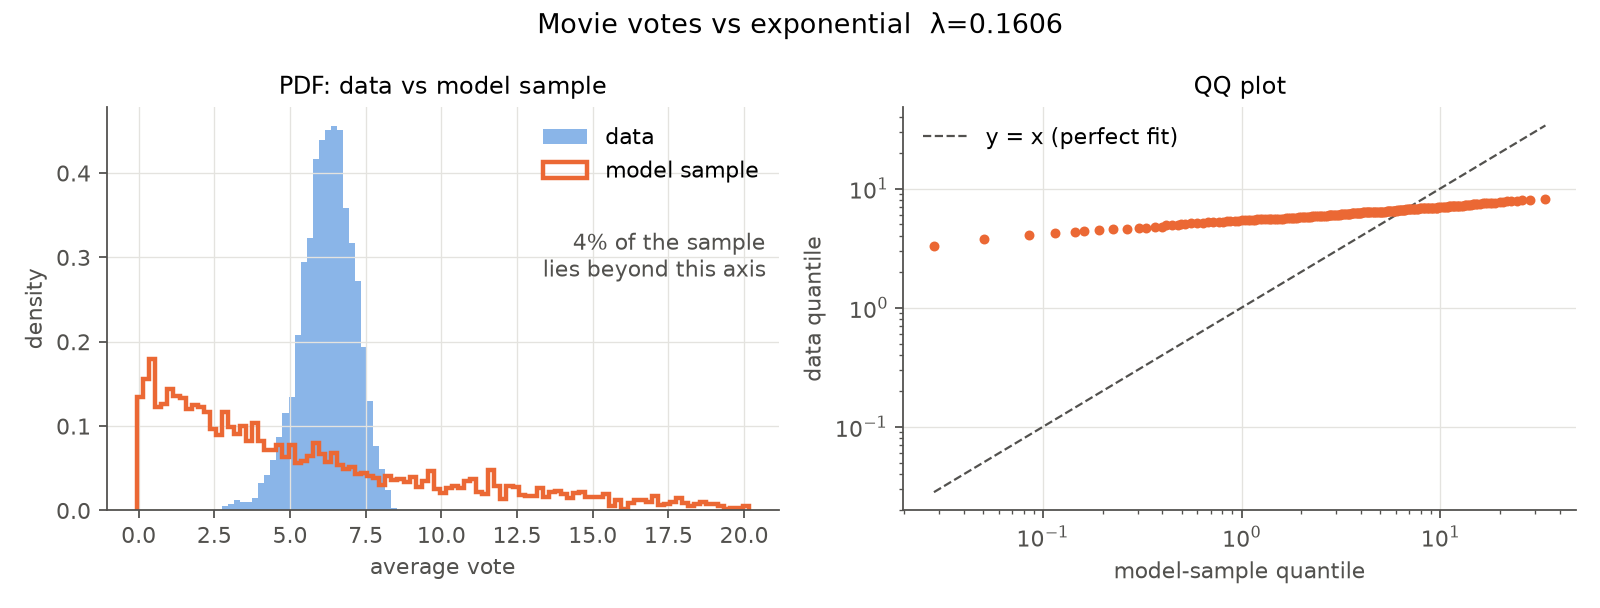
\includegraphics[width=\linewidth]{../figures/p1b_2_exponential.png}
  \caption{영화 평점에 지수분포($\hat\lambda = 0.1606$)를 적합한 결과
  (\texttt{code/p1.py}가 생성). $D = 0.490$.}
  \label{fig:p1b-exp}
\end{figure}

\end{document}
